\chapter[Resultados Obtidos]{Resultados Obtidos}
Neste capítulo serão exibidos os resultados obtidos nesta primeira parte do projeto. Será falado dos resultados sobre o software de extração e da plataforma web.
\section{Software de Extração}
Na parte de extração dos dados foram criados dois codigos teste. O código \ref{code:handler} representa o uso da \textit{gem} \textit{clockwork} como um \textit{handler} de frequência, o resultado obtido pelo uso do código pode ser visto na figura \ref{image:result_handler}. Já o código \ref{code:plugin} representa uma estrutura inicial de um \textit{plugin}, nele é feito a conexão com o Elasticsearch, extraídos os dados de uma API, manipula esses dados e inserir no Elasticsearch.
\begin{lstlisting}[language={Ruby}, caption = {Código do \textit{Handler}}, label = {code:handler}]
require 'clockwork'
require 'active_support/time'

# O modulo necessita ter o nome Clockwork
module Clockwork

	count_frequency = 0
	count_games = 0

	# Handler dos jobs
	handler do |job|
		if job.eql? 'frequency'
			count_frequency += 1
			print "A frequencia e: #{count_frequency}\n"
		elsif job.eql? 'games'
			count_games += 1
			print "O numero de jogos e: #{count_games}\n"
		end
	end

	# Define a frequencia dos jobs
	every(30.seconds, 'frequency')
	every(1.minutes, 'games')
end
\end{lstlisting}
\begin{figure}
\centering
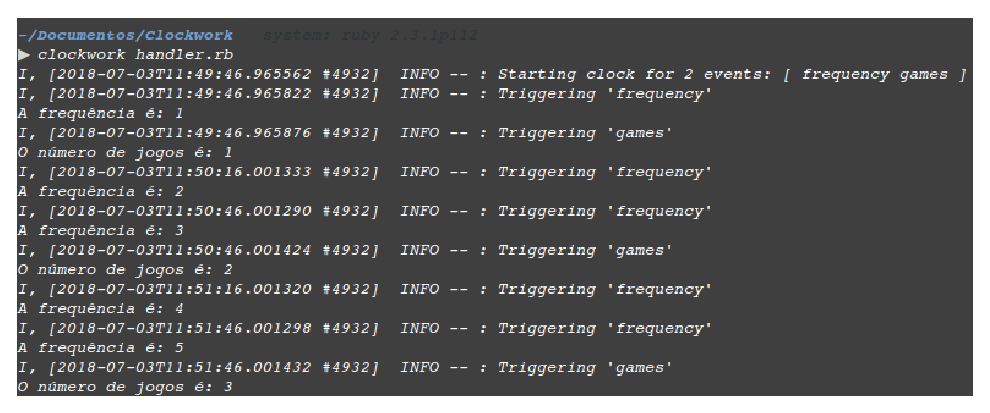
\includegraphics[scale=0.6]{figuras/result_handler.eps}
\caption{Resultado da Compilação do \textit{Handler}}
\label{image:result_handler}
\end{figure}
\begin{lstlisting}[language={Ruby}, caption = {Código do \textit{Plugin}}, label = {code:plugin}]
require 'httparty'
require 'elasticsearch'

# Classe que funciona como uma hash
class Game < Hash
	def put(key, value)
		self[key] = value;
	end
end

game = Game.new
# Conecta com o Elasticsearch
client = Elasticsearch::Client.new log: true
# Verifica se aquele index ja existe
if !client.indices.exists? index: 'test'
	client.indices.create index: 'test'
end
id = 730
url = 'http://store.steampowered.com/api/appdetails/?appids=' + id.to_s
# Extrai dados da API
response = HTTParty.get(url)
response.parsed_response
data = response["730"]["data"]
game.put("name", data["name"])
game.put("description", data["detailed_description"])
# Insere os dados no Elasticsearch
client.update index: 'test', type: 'game', id: 730, body: game.to_json
\end{lstlisting}
No decorrer do desenvolvimento da primeira parte do projeto, houve um mudança na política de privacidade da Steam, e isso modificou alguns dados que seriam extraídos, o principal foi o de número de donos. Antes de mudança a API do Steam Spy, providenciava um número quase exato do número de donos, após a mudança, agora a API providência apenas uma média estimada do número de donos. Isto alterar o projeto, já que agora não e possível mais fazer uma métrica exata da média de donos daquele gênero.
\section{Plataforma Web}
Para a plataforma web foi criado um protótipo que exibe como será a visualização dos dados, é também como será o fluxo dentro da plataforma. A figura \ref{image:inicial} é a tela inicial da plataforma, dela pode-se ir para as métricas ou para a aba sobre. A figura \ref{image:metrics} é a tela onde será apresentada as métricas, nesta página o usuário poderá definir os gêneros e as categorias que definirão o perfil do jogo. A figura \ref{image:rankings} é a tela quando o usuário clica na aba \textit{rankings}, nesta aba serão exibidas os \textit{rankings} de jogos daquele determinado perfil. A figura \ref{image:sugestoes} é a tela quando o usuário clica na aba sugestões, nesta aba serão exibidas algumas sugestões para a evolução daquele perfil.
\begin{figure}
\centering
\includegraphics[scale=0.3]{figuras/tela_inicial.eps}
\caption{Tela Inicial}
\label{image:inicial}
\end{figure}
\begin{figure}
\centering
\includegraphics[scale=0.3]{figuras/tela_metrics.eps}
\caption{Tela de Métricas}
\label{image:metrics}
\end{figure}
\begin{figure}
\centering
\includegraphics[scale=0.3]{figuras/tela_ranking.eps}
\caption{Tela de \textit{Rankings}}
\label{image:rankings}
\end{figure}
\begin{figure}
\centering
\includegraphics[scale=0.3]{figuras/tela_sugestoes.eps}
\caption{Tela de Sugestões}
\label{image:sugestoes}
\end{figure}
O protótipo poderá ser visualizado no seguinte \textit{link}: \url{https://marvelapp.com/3209ad6}.